\section{Proposed Approach}
\label{sec:propo_approch}
Following the rationale in \cite{deyPassivityBasedDecentralizedCriteria2023} and \cite{chenExtendedFrequencyDomainPassivity2025a}, we show that sectoriality is not an intrinsic property of the system, but rather depends on the specific selection of inputs and outputs. Consequently, an alternative choice of variables may enable the system to exhibit sectoriality.

\subsection{Power-Polar coordinates frame}
A particularly suitable choice for GFM converters is to represent voltages in power-polar coordinates, i.e., using voltage magnitude and phase as inputs, and active and reactive power as outputs. As demonstrated in \cite{deyAnalysisPassivityCharacteristics2021}, this representation yields a passive mapping for GFM converters in the low-frequency range, and therefore a sectorial system. For each converter $i$, the associated linearized change of variables is given by \eqref{eq:change_of_coord_1}–\eqref{eq:change_of_coord_2}, where the transformation matrices $\mathcal{E}_i$, $\mathcal{F}_i$, and $\mathcal{C}_i$ depend on the voltage and current operating point.
\begin{equation}
    \begin{bmatrix}
        \phi_i \\ |V|_i 
    \end{bmatrix} =
    \underbrace{\begin{bmatrix}
        -V^i_{q,0} & \frac{V^i_{d,0}}{\sqrt{(V^i_{d,0})^2+(V^i_{q,0})^2}} \\
        V^i_{q,0} & \frac{V^i_{q,0}}{\sqrt{(V^i_{d,0})^2+(V^i_{q,0})^2}}
    \end{bmatrix}}_{:=\mathcal{F}_i^{-1}}
    \begin{bmatrix}
        V_{D,i} \\ V_{Q,i} 
    \end{bmatrix}
    \label{eq:change_of_coord_1}
\end{equation}

\begin{equation}
    \begin{bmatrix}
        P_i \\ Q_i
    \end{bmatrix} = \underbrace{\begin{bmatrix}
        V^i_{d,0} & V^i_{q,0}  \\
        V^i_{q,0} & -V^i_{d,0}
    \end{bmatrix}}_{:=\mathcal{E}_i} \begin{bmatrix}
        I_{D,i} \\ I_{Q,i} 
    \end{bmatrix} + 
    \underbrace{\begin{bmatrix}
        I^i_{d,0} & V^i_{q,0}  \\
        -I^i_{q,0} & I^i_{d,0}
    \end{bmatrix}}_{:=\mathcal{C}_i}
    \begin{bmatrix}
        V_{D,i} \\ V_{Q,i} 
    \end{bmatrix}
    \label{eq:change_of_coord_2}
\end{equation}

With these definitions, the converter’s new input–output relation becomes as in \eqref{eq:pp_trasnf} and similar the transformation is applied to the network, yielding \eqref{eq:pp_trasnf_net}.
\begin{equation}
    J_{C,i}(s) :=(\mathcal{E}_iY_{C_i}(s)+\mathcal{C}_i)\mathcal{F}_i
    \label{eq:pp_trasnf}
\end{equation}
\begin{equation}
    \mathbf{J}_{net}(s) :=(\boldsymbol{\mathcal{E}}\mathbf{Y}_{net}(s)-\boldsymbol{\mathcal{C}})\boldsymbol{\mathcal{F}}
    \label{eq:pp_trasnf_net}
\end{equation}
$\boldsymbol{\mathcal{E}}$, $\boldsymbol{\mathcal{C}}$ and $\boldsymbol{\mathcal{F}}$ are the block-diagonal matrices build from $\mathcal{E}_i$, $\mathcal{C}_i$ and $\mathcal{F}_i$, respectively. The minus sign in $\mathcal{C}$ comes from the fact that the current in the network flows in the opposite direction to that assumed in the converter. We denote $\mathbf{J}_C$ the block-diagonal matrix build from $J_{C_i}$ as in \eqref{eq:block_diagonal}.

This change of variables can be interpreted as a loop transformation, as illustrated in Fig. \ref{fig:loop_shaping}. 
Assuming the transformation is well-defined, input/output stability of the transformed system and the original system are equivalent. Indeed, the stability is determined by the zeros of $\det(\mathbf{Y}_{net}(s)+\mathbf{Y}_C(s))$. Since $\det(\mathbf{J}_C(s) +\mathbf{J}_{net}) = \det(\boldsymbol{\mathcal{E}}(\mathbf{Y}_{net}(s)+\mathbf{Y}_{C}(s))\boldsymbol{\mathcal{F}})$, the zeros of the transformed system and the original are identical. Moreover, if there are no right plane pole/zero cancellations, then
 input–output stability implies internal stability, as shown for instance in \cite{häberle2025decentralizedparametricstabilitycertificates}. Theorem \ref{thm:dec_mixed_small_gain_phase} can be applied directly to the transformed system without loss of generality.

\begin{figure}
    \centering
    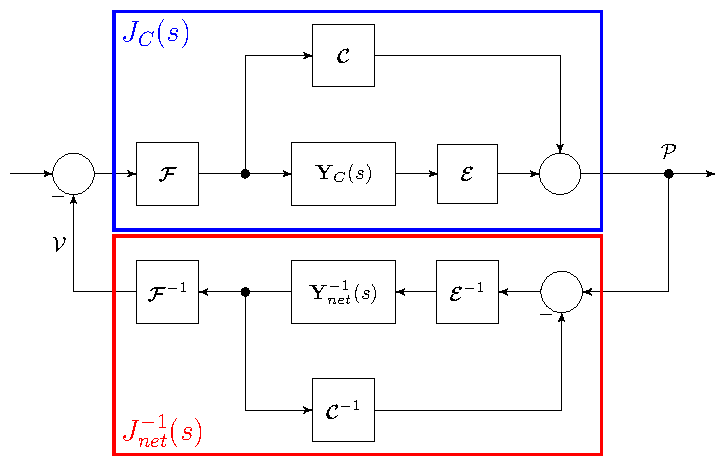
\includegraphics[width=\linewidth]{loop_shaping.pdf}
    \caption{Proposed transformation as loop-shaping transformation}
    \label{fig:loop_shaping}
\end{figure}

\begin{rem}
    The proposed transformation 
    %generalizes the post-multiplication approach introduced in 
    combines the post-multiplication and the shaping functions from \cite{woolcockMixedGainPhase2023, chenExtendedFrequencyDomainPassivity2025a, deyPassivityBasedDecentralizedCriteria2023}. In \eqref{eq:pp_trasnf}, both pre- and post-multiplication are performed, along with a translation term $\mathcal{C}$.
\end{rem}
Taking in consideration the GFM model introduced in \eqref{eq:frame_embedding} and applying the transformation, a straightforward computation shows that $J_C(s)$ evaluated at 0 is equal to \eqref{eq:J_C_0}, for some scalar $\gamma$. Indeed, in this formulation a phase jump does not produce any steady-state power deviation, while a deviation in voltage magnitude results only in a change in reactive power. 
It is a diagonal matrix with eigenvalues $0$ and $\gamma$, and its numerical range is a straight segment connecting this two eigenvalues. 
\begin{equation}
    J_C(0)=\begin{bmatrix}
        0 & 0 \\
        0 & \gamma \\
    \end{bmatrix}
    \label{eq:J_C_0}
\end{equation}

In this frame, the converter admittance at zero frequency is quasi-sectorial with a well-defined phase. While this may not extend across the low-frequency range, it remains a promising indication.
Nevertheless, for the small-phase criterion to be applicable, sectoriality must hold across the entire frequency range for both $\mathbf{J}_C(s)$, and $\mathbf{J}^{-1}_{net}(s)$. 
While the transformation can resolve the low-frequency non-sectoriality, it does not guarantee that sectoriality will persist at higher frequencies.

To illustrate this point, the same analysis as before is repeated for a GFM connected to an infinite bus. The small-phase criteria is shown in Figure \ref{fig:pp_frame_cond}. The converter exhibits sectorial behavior up to approximately $64$ Hz, within which the small-phase condition is satisfied. Beyond this frequency, neither the converter nor the network remain sectorial, rendering the criterion inapplicable. This highlights that, while the transformation addresses the dominant low-frequency limitation, it does not fully eliminate the applicability restrictions of the small-phase approach.

\begin{rem}
    Although $\mathbf{J}_C(s)$ inherits stability from $\mathbf{Y}_C(s)$, the same cannot be guaranteed for $\mathbf{J}^{-1}_{net}(s)$. The associated transformation can be interpreted as a feedback operation, which may potentially destabilize the system. Consequently, prior to applying Theorem \ref{thm:dec_mixed_small_gain_phase}, the stability of $\mathbf{J}^{-1}_{net}(s)$ must be verified.
\end{rem}

\begin{figure}
    \centering
    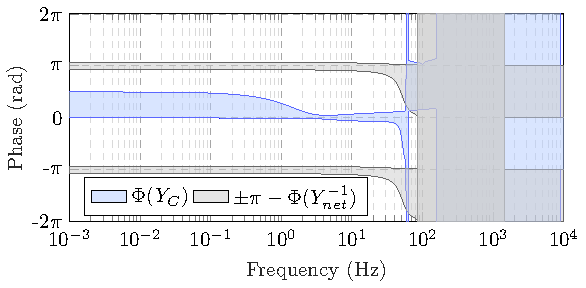
\includegraphics[width=\linewidth]{Phase_polar.pdf}
    \caption{Small phase condition for a GFM converter in Power-Polar frame}
    \label{fig:pp_frame_cond}
\end{figure}

\subsection{Unified Approach}
As shown in the previous section, neither the criteria in the standard rectangular admittance frame nor those in the power–polar frame are satisfied across the entire frequency range.
In the rectangular frame, the phase remains well-defined and the small-phase condition is fulfilled at high frequencies (e.g., $f>0.7$ Hz). In contrast, for the loop-shaped system in the polar frame, the phase is well-defined and the small-phase condition is satisfied at low frequencies (e.g., $f<64$ Hz).

An intuitive approach might be to combine the two frames: use the rectangular frame phase at high frequencies and the polar-frame phase at low frequencies, and declare the system stable if the small-phase criterion is satisfied in at least one frame at each frequency. However, it is possible to construct a counterexample demonstrating that stability cannot be inferred simply by merging frequency-wise results from different frames.
The fundamental reason lies in the fact that different transformations bound different quantities:
the eigenvalues of $\mathbf{J}_C(j\omega)\mathbf{J}^{-1}_{net}(j\omega)$ are, in general, not the same as those of $\mathbf{Y}_C(j\omega)\mathbf{Y}^{-1}_{net}(j\omega)$ if $\mathcal{C}$ is different from the zero matrix.

%One possible solution is to define a generic transformation, parameterized by the matrices $\mathcal{E}_i$, $\mathcal{F}_i$, and $\mathcal{C}_i$ such that sectoriality is ensured across the entire frequency range. This concept is further extended to frequency-dependent matrices, as expressed in \eqref{eq:generic_trasnf}.

To merge these two frames into a single system, we consider the shaping matrices $\mathcal{E}_i$, $\mathcal{F}_i$, and $\mathcal{C}_i$ to be frequency-dependent matrices, as expressed in \eqref{eq:generic_trasnf}.

\begin{equation}
\begin{aligned}
    &\tilde{J}_{C_i}(s) =(\mathcal{E}_i(s)Y_{C_i}(s)+\mathcal{C}_i(s))\mathcal{F}_i(s) \\
    &\tilde{\mathbf{J}}_{net}(s) =(\boldsymbol{\mathcal{E}}(s)\mathbf{Y}_{net}(s)-\boldsymbol{\mathcal{C}}(s))\boldsymbol{\mathcal{F}}(s)
    \label{eq:generic_trasnf}
\end{aligned}
\end{equation}
These matrices must be selected so that each $\tilde{J}_{C_i}(s)$ and $\tilde{\mathbf{J}}^{-1}_{net}(s)$ are stable.
Moreover, if the shaping matrices $\boldsymbol{\mathcal{E}}(s)$, $\boldsymbol{\mathcal{C}}(s)$ and $\boldsymbol{\mathcal{F}}(s)$ are well-posed, the stability of the loop-shaped system composed of $\tilde{\mathbf{J}}_{c}$ and $\tilde{\mathbf{J}}_{net}$ is equal to the stability of the original system composed by $\mathbf{Y}_{c}$ and $\mathbf{Y}_{net}$. 
This formulation provides significant flexibility in choosing the transformation matrices, but identifying ones that simultaneously ensure open-loop stability and sectoriality over the full frequency range is nontrivial.

%Therefore, we propose a different formulation with an added degree of freedom that helps us satisfy the sectoriality assumption for practical examples"  + getting good bounds 

Ideally, at low frequencies the matrices should correspond to those in \eqref{eq:change_of_coord_1}-\eqref{eq:change_of_coord_2} (denoted from now on as $\mathcal{E}_{J,i}$, $\mathcal{F}_{J,i}$ and $\mathcal{C}_{J,i}$), while at high frequencies they should revert to the rectangular frame (i.e., $\mathcal{E}=\mathcal{F}=I$ and $\mathcal{C}=0$, denoted from now on as $\mathcal{E}_{Y,i}$, $\mathcal{F}_{Y,i}$ and $\mathcal{C}_{Y,i}$). A continuous transition between these two regimes is necessary. A trivial choice for $\mathcal{E}_i(s)$, and similar for $\mathcal{F}_i(s)$ and $\mathcal{C}_i(s)$, can be as in \eqref{eq:freq_dep_tf} using an low/high-pass filtering approach. 
The filters transfer function are given as: $H_{LPF}(s)=w_c/(s+w_c)$ and $H_{HPF}(s)=1-H_{LPF}(s)$, with $w_c$ the filter cut-off frequency. 
\begin{equation}
    \mathcal{E}_i(s) = H_{LPF}(s)\mathcal{E}_{J,i}+H_{HPF}(s)\mathcal{E}_{Y,i}
    \label{eq:freq_dep_tf}
\end{equation}
This transformation proves in general inadequate since sectoriality is lost near the filter cut-off frequency $w_c$. 
%This is because when the filter start to effect the transformed system, the numerical range starts to rotate and at some point it incorporates the origin. 
To ensure sectoriality while obtaining tight phase bounds, we propose instead the transformation in~\eqref{eq:freq_dep_tf_better}, with an additional degree of freedom $W_i$. In this formulation, frequency-dependent filtering is applied exclusively to $\mathcal{C}$ and $\mathcal{F}(s)$, while $\mathcal{E}(s)$ remains constant.
\begin{equation}
\begin{aligned}
    &\mathcal{E}_i(s) = \mathcal{E}_{J,i} \\
    &\mathcal{C}_i(s) = H_{LPF}(s)\mathcal{C}_{J,i}\\
    &\mathcal{F}_i(s) = H_{LPF}(s)\mathcal{F}_{J,i}+H_{HPF}(s)W_i(s)\mathcal{E}_{J,i}^{-1}
\end{aligned}
\label{eq:freq_dep_tf_better}
\end{equation}
%Assume for the moment that $W_i(s)$ is the identity matrix. The rationale behind the particular choice, even if we do not filter $\mathcal{E}_i$, at high frequency we obtain $J_{C_i}\approx\mathcal{E}_{J,i}Y_{C_i}\mathcal{E}_{J,i}^{-1}$, and since a similarly transformation does not change the numerical range, we get back the rectangular frame.
From practical observation, this transformation compared to \eqref{eq:freq_dep_tf} provides smooth transitions between the two frames, and sectoriality is easier to obtain.
For instance, setting $W_i(s)$ equal to the identity matrix
let us recover the rectangular frame at high frequencies, since $J_{C_i}\approx\mathcal{E}_{J,i}Y_{C_i}\mathcal{E}_{J,i}^{-1}$ (and a similarly transformation does not change the numerical range). $W_i(s)$ is an additional weighted matrix  introducing further flexibility to, for example, transfer known dynamics from $Y_{C_i}(s)$ to $\mathbf{Y}_{net}(s)$, eventually allowing better sectorial behavior and stricter phase bounds. This concept is clarified in the next section with an example. Nonetheless, other transformations may ensure sectoriality and tight phase bounds; finding out an optimal loop-shaping transformation is still an open point.